%!TEX root = constraint-layout.tex

% \newcommand{\teaserFigure}{
% 	\teaser{
% 		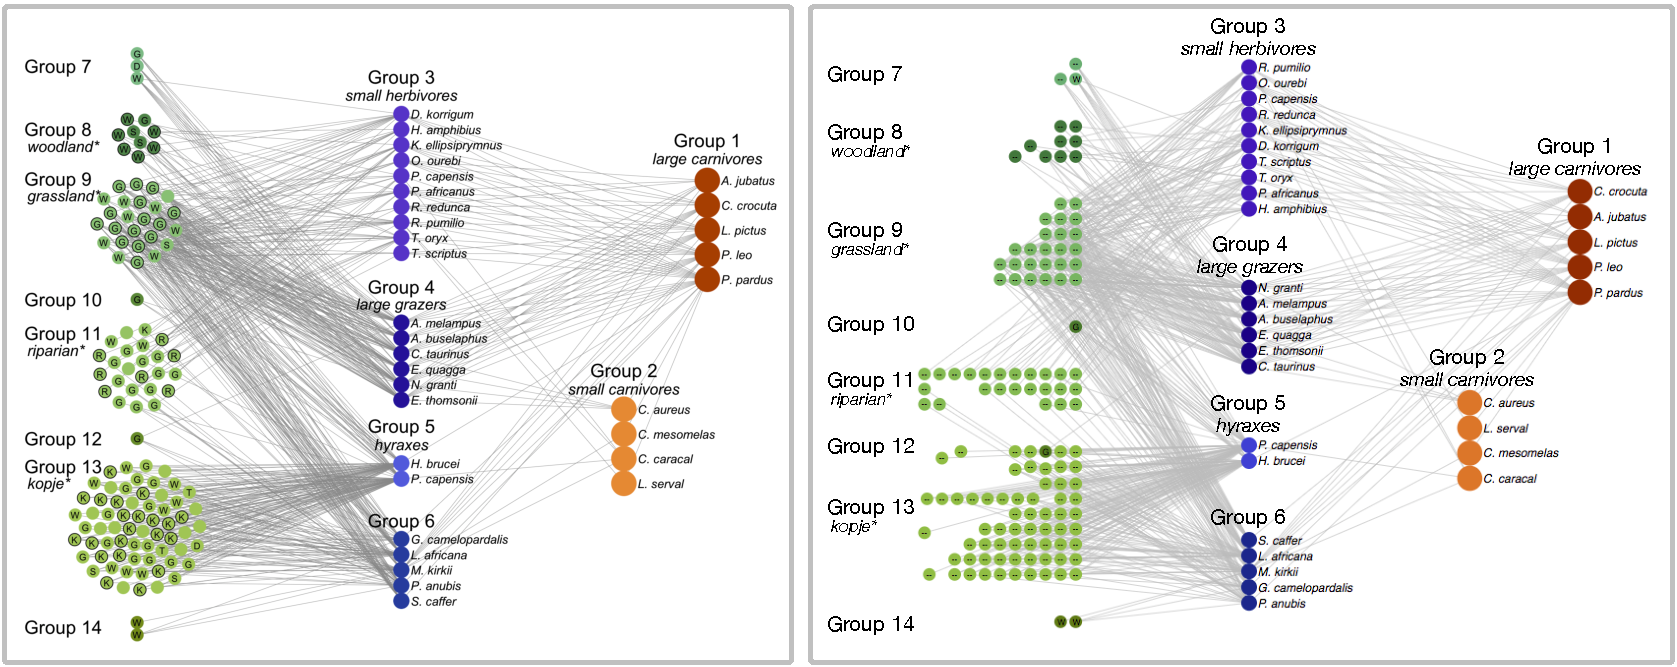
\includegraphics[width=\linewidth]{figures/serengeti-layout.pdf}
% 		\centering
% 	  \caption{\label{fig:teaser}}

% 	}
% }

\newcommand{\serengetiLayoutColumn}{
  \begin{figure}[t!]
    \centering
    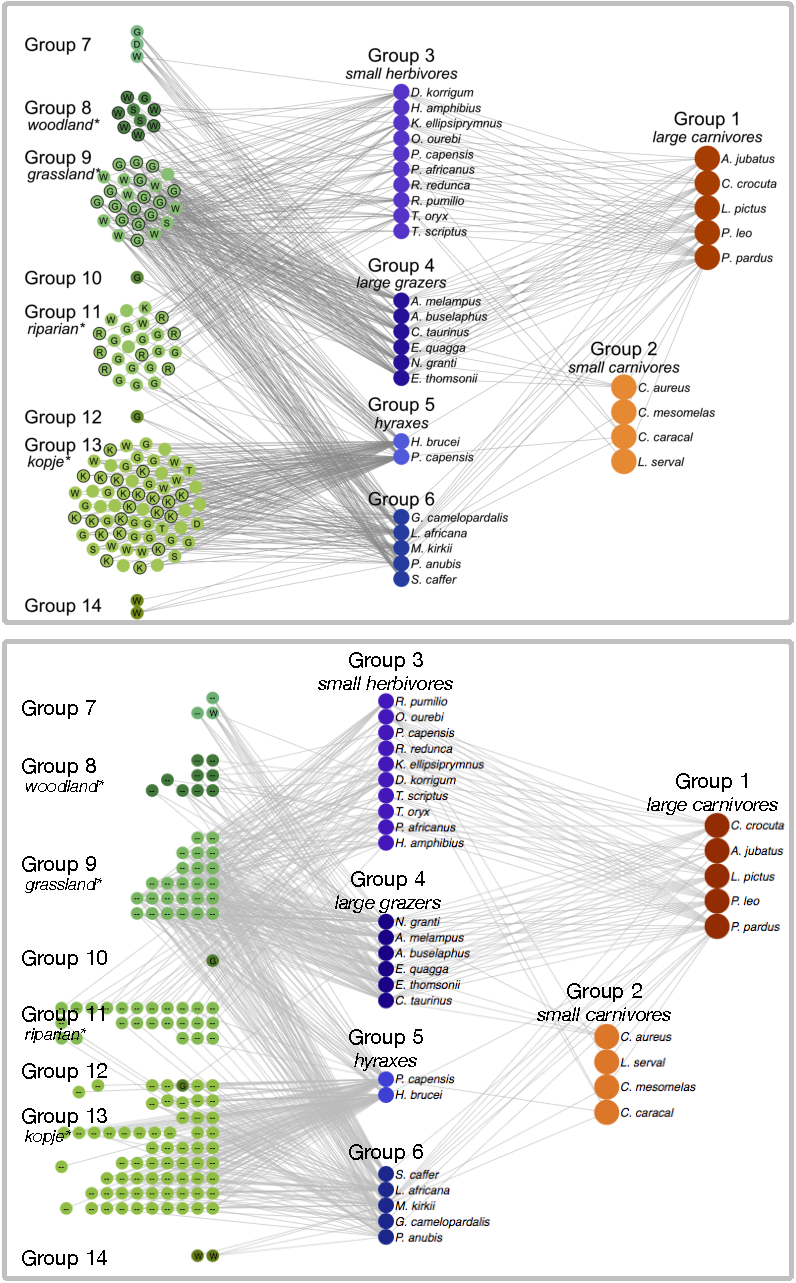
\includegraphics[width=0.81\columnwidth]{figures/serengeti-layout-column.pdf}
    {\caption{\label{fig:serengeti-layout}
    The layout for the Serengeti food web using our constraint language, as compared to Baskerville et al. \cite{baskerville2011spatial}.}}
    \vspace{-40px}
  \end{figure}
}

%%%%%%%%%%%%%%%%%%%%%%%%%%%%%%%%%%
%%%%%%%%%%%%% Design %%%%%%%%%%%%%
%%%%%%%%%%%%%%%%%%%%%%%%%%%%%%%%%%

\newcommand{\smallTreeExample}{
  \begin{figure}[t!]
    \centering
    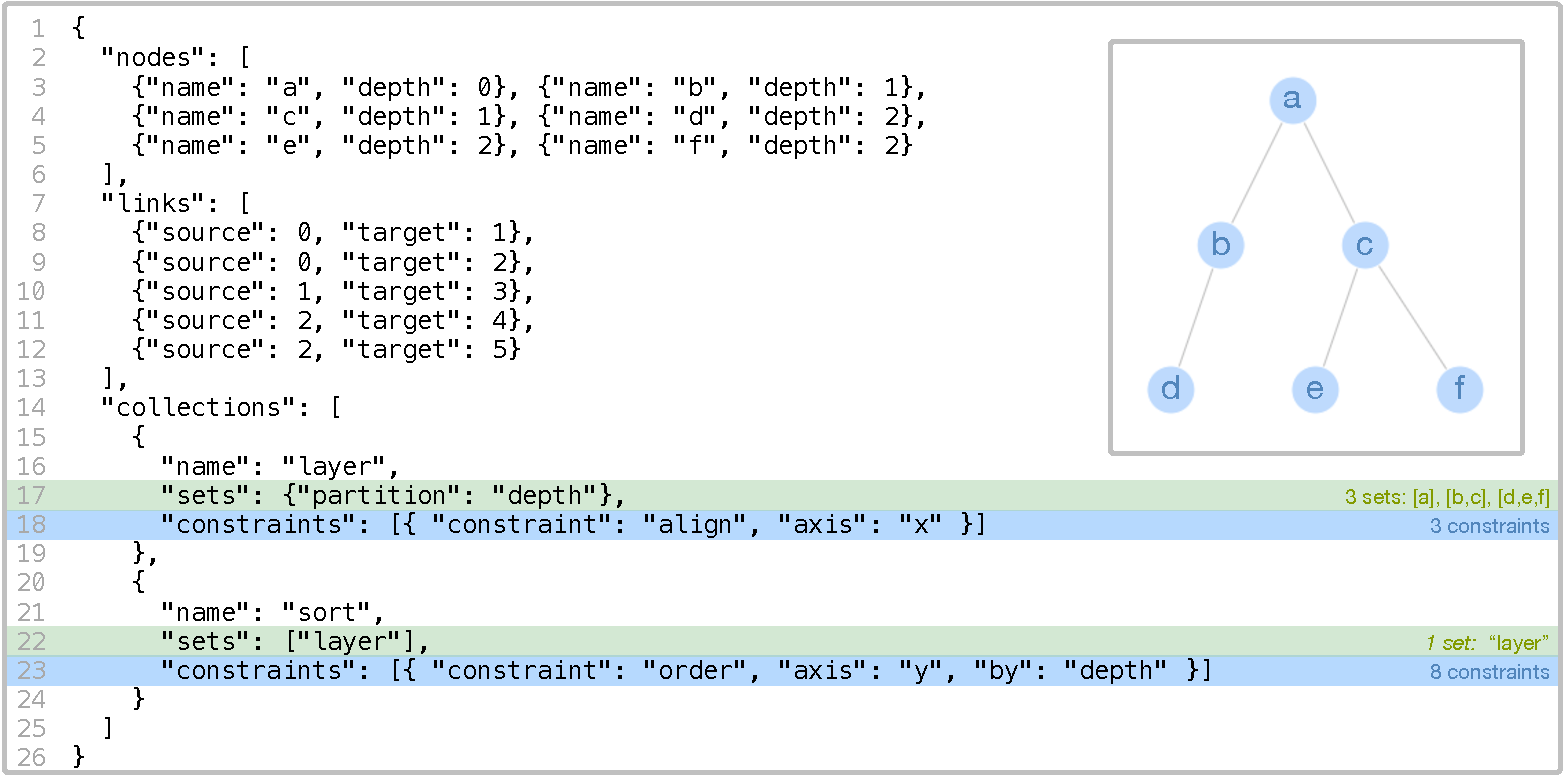
\includegraphics[width=\columnwidth]{figures/small-tree-example.pdf}
                    {\caption{\label{fig:small-tree-example} The full
                        \projectname\ specification for a small tree with
                        six nodes. Nodes are split into sets based on their
                        depth from the root \texttt{a}, and aligned. A new
                        collection is formed containing the ``layer'' set
                        and the layers are ordered by their depth to form
                        the tree.  }}
    \vspace{-20px}
  \end{figure}
}

\newcommand{\contradictionExample}{
  \begin{figure}[t!]
    \centering
    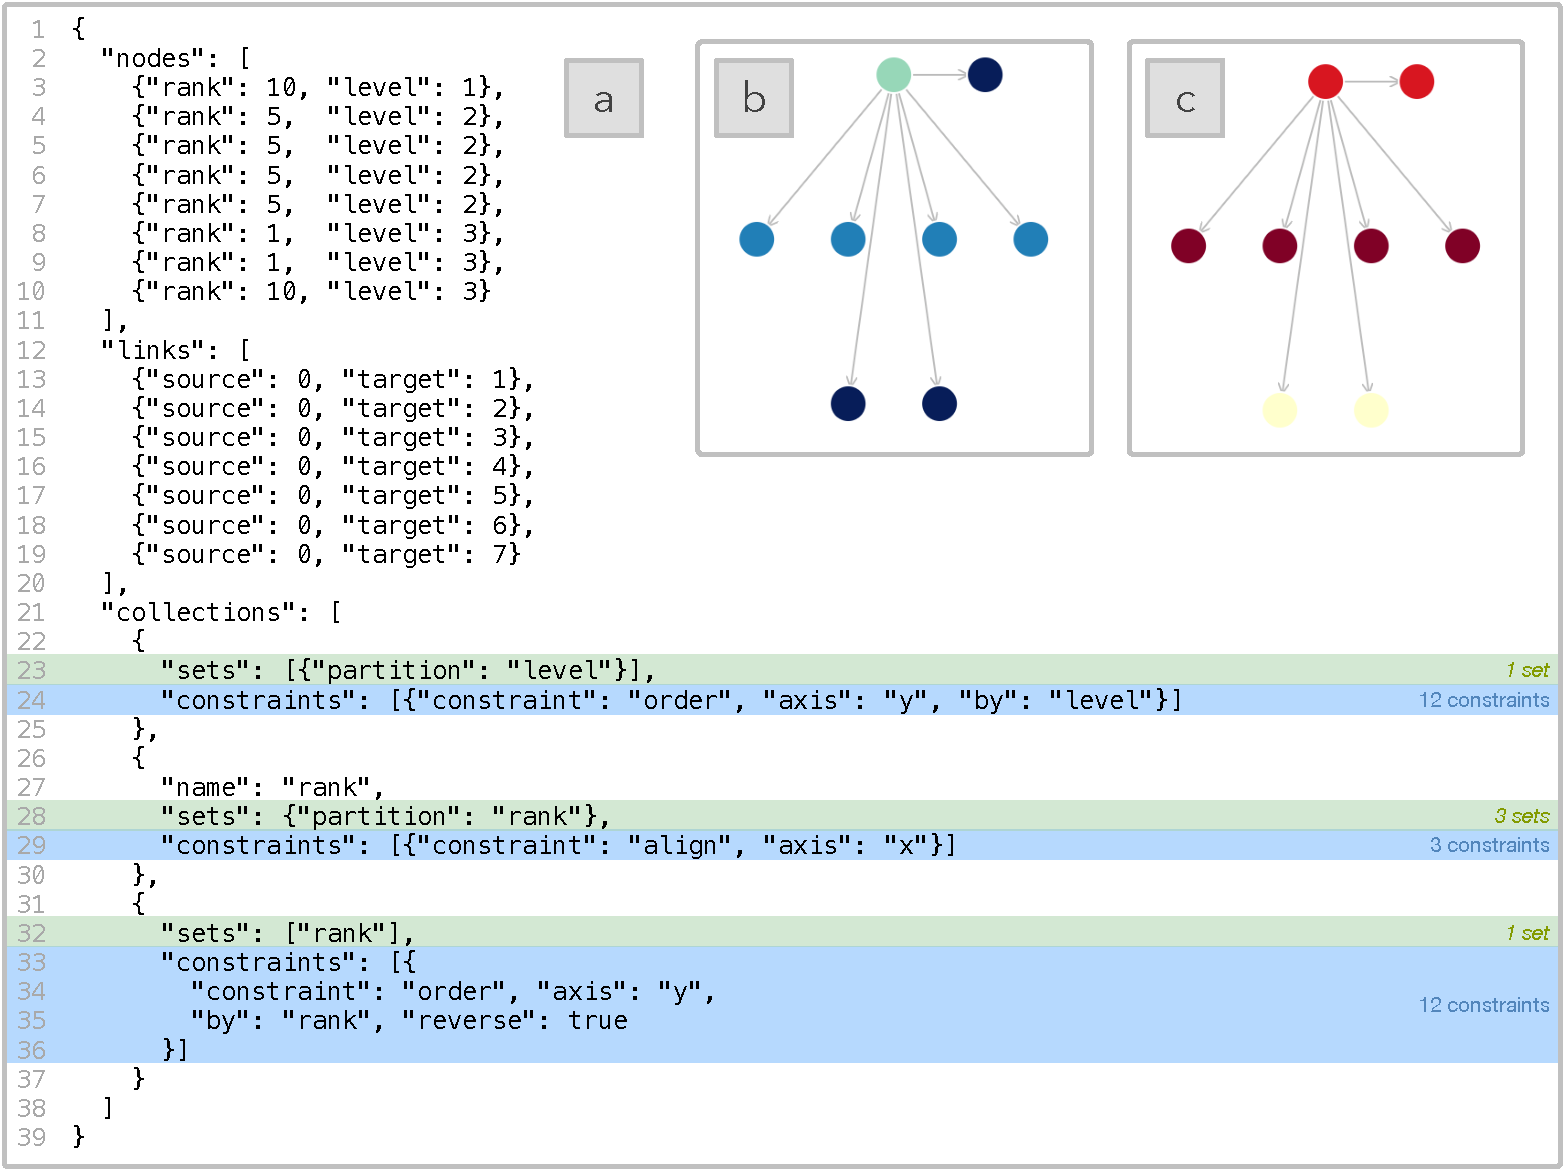
\includegraphics[width=\columnwidth]{figures/contradiction-example.pdf}
                    {\caption{\label{fig:contradiction-example} (a) The
                        full \projectname\ specification for a small graph
                        with eight nodes. (b) Nodes are aligned based on
                        their \texttt{rank}, and colored based on their
                        \texttt{level}. Two constraints are applied to
                        order the nodes, once by \texttt{level} and once by
                        \texttt{rank}, which produces a contradiction. (c)
                        Nodes are colored based on the amount of error for
                        constraints that are invalid.  }}
    \vspace{-20px}
  \end{figure}
}

%%%%%%%%%%%%%%%%%%%%%%%%%%%%%%%%%%
%%%%%%%%% Demonstration %%%%%%%%%%
%%%%%%%%%%%%%%%%%%%%%%%%%%%%%%%%%%

\newcommand{\krugerLayout}{
  \begin{figure}[t!]
    \centering
    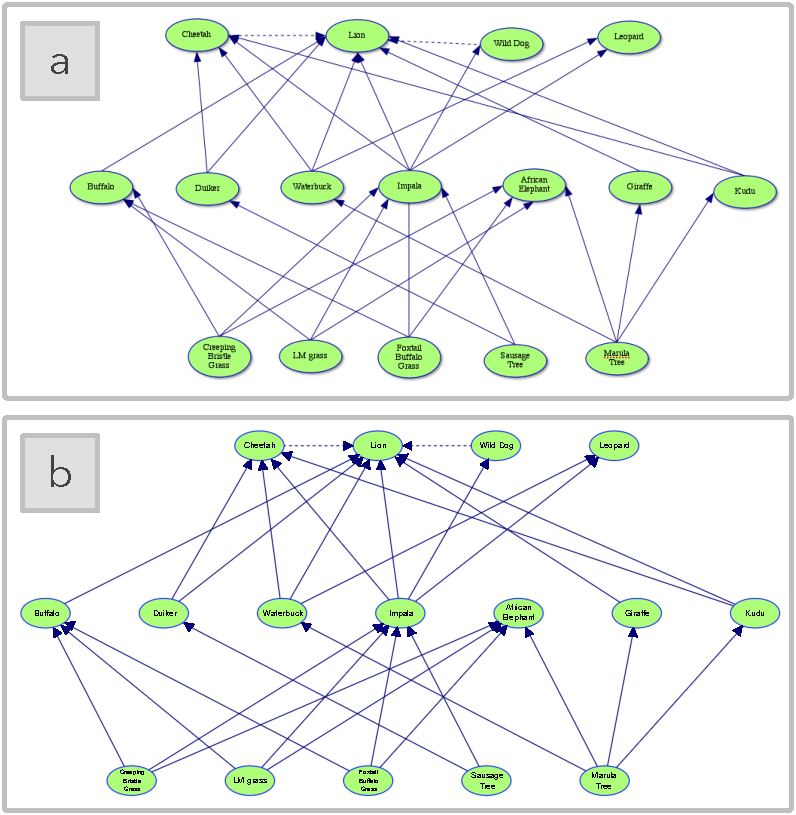
\includegraphics[width=0.81\columnwidth]{figures/kruger-layout.pdf}
                    {\caption{\label{fig:kruger-layout} The layout for a
                        small subset of the food web for Kruger National
                        Park from (a) their website \orange{citation} as
                        compared to (b) our layout using \projectname.}}
    \vspace{-20px}
  \end{figure}
}

\newcommand{\serengetiLayout}{
  \begin{figure*}[t]
    \centering
    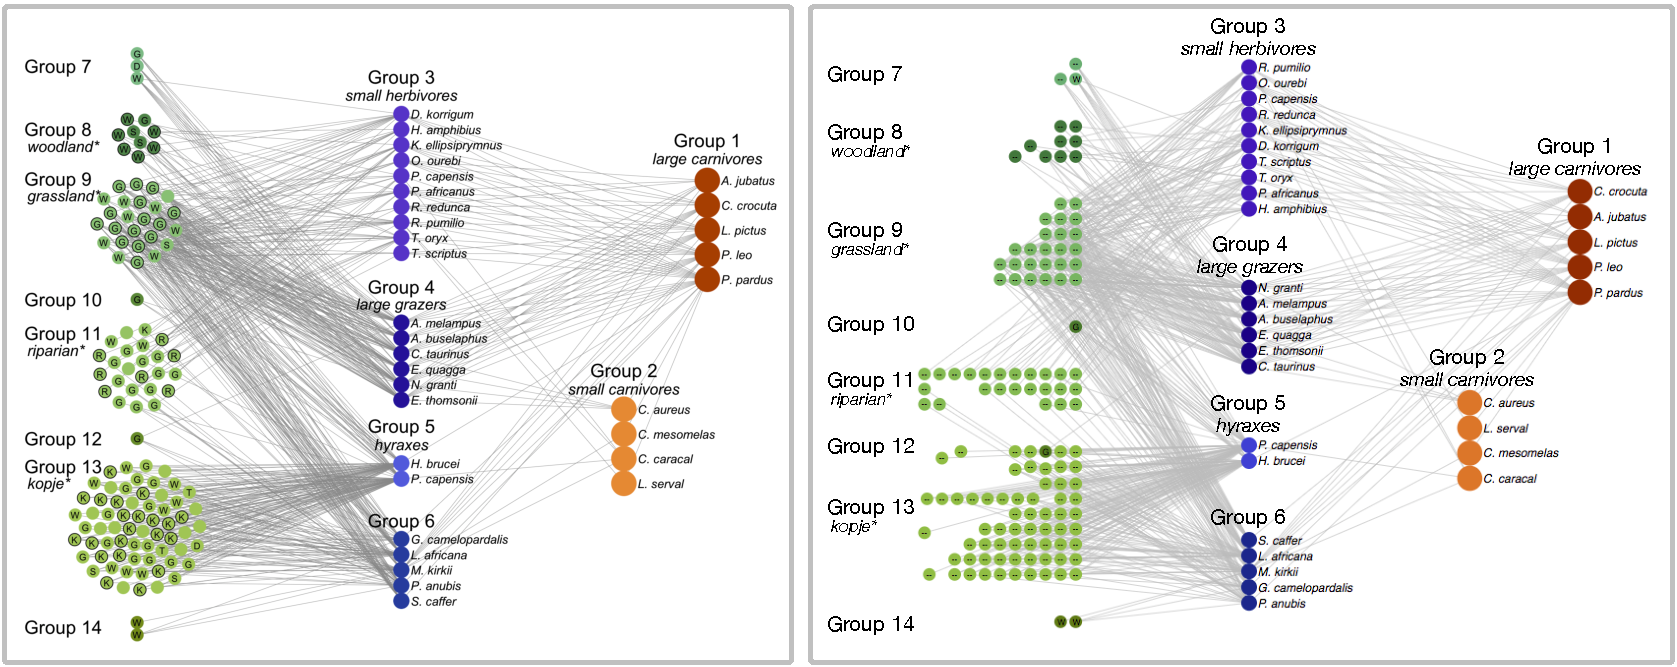
\includegraphics[width=\textwidth]{figures/serengeti-layout.pdf}
    \vspace{-20px} {\caption{\label{fig:serengeti-layout} The layout for
        the Serengeti food web using our constraint language, as compared
        to Baskerville et al. \cite{baskerville2011spatial}. \todo{retake
          photos on retina screen} \todo{label the two sides of the figure
          a/b}}}
  \end{figure*}
}

\newcommand{\serengetiSpec}{
  \begin{figure}[t]
    \centering
    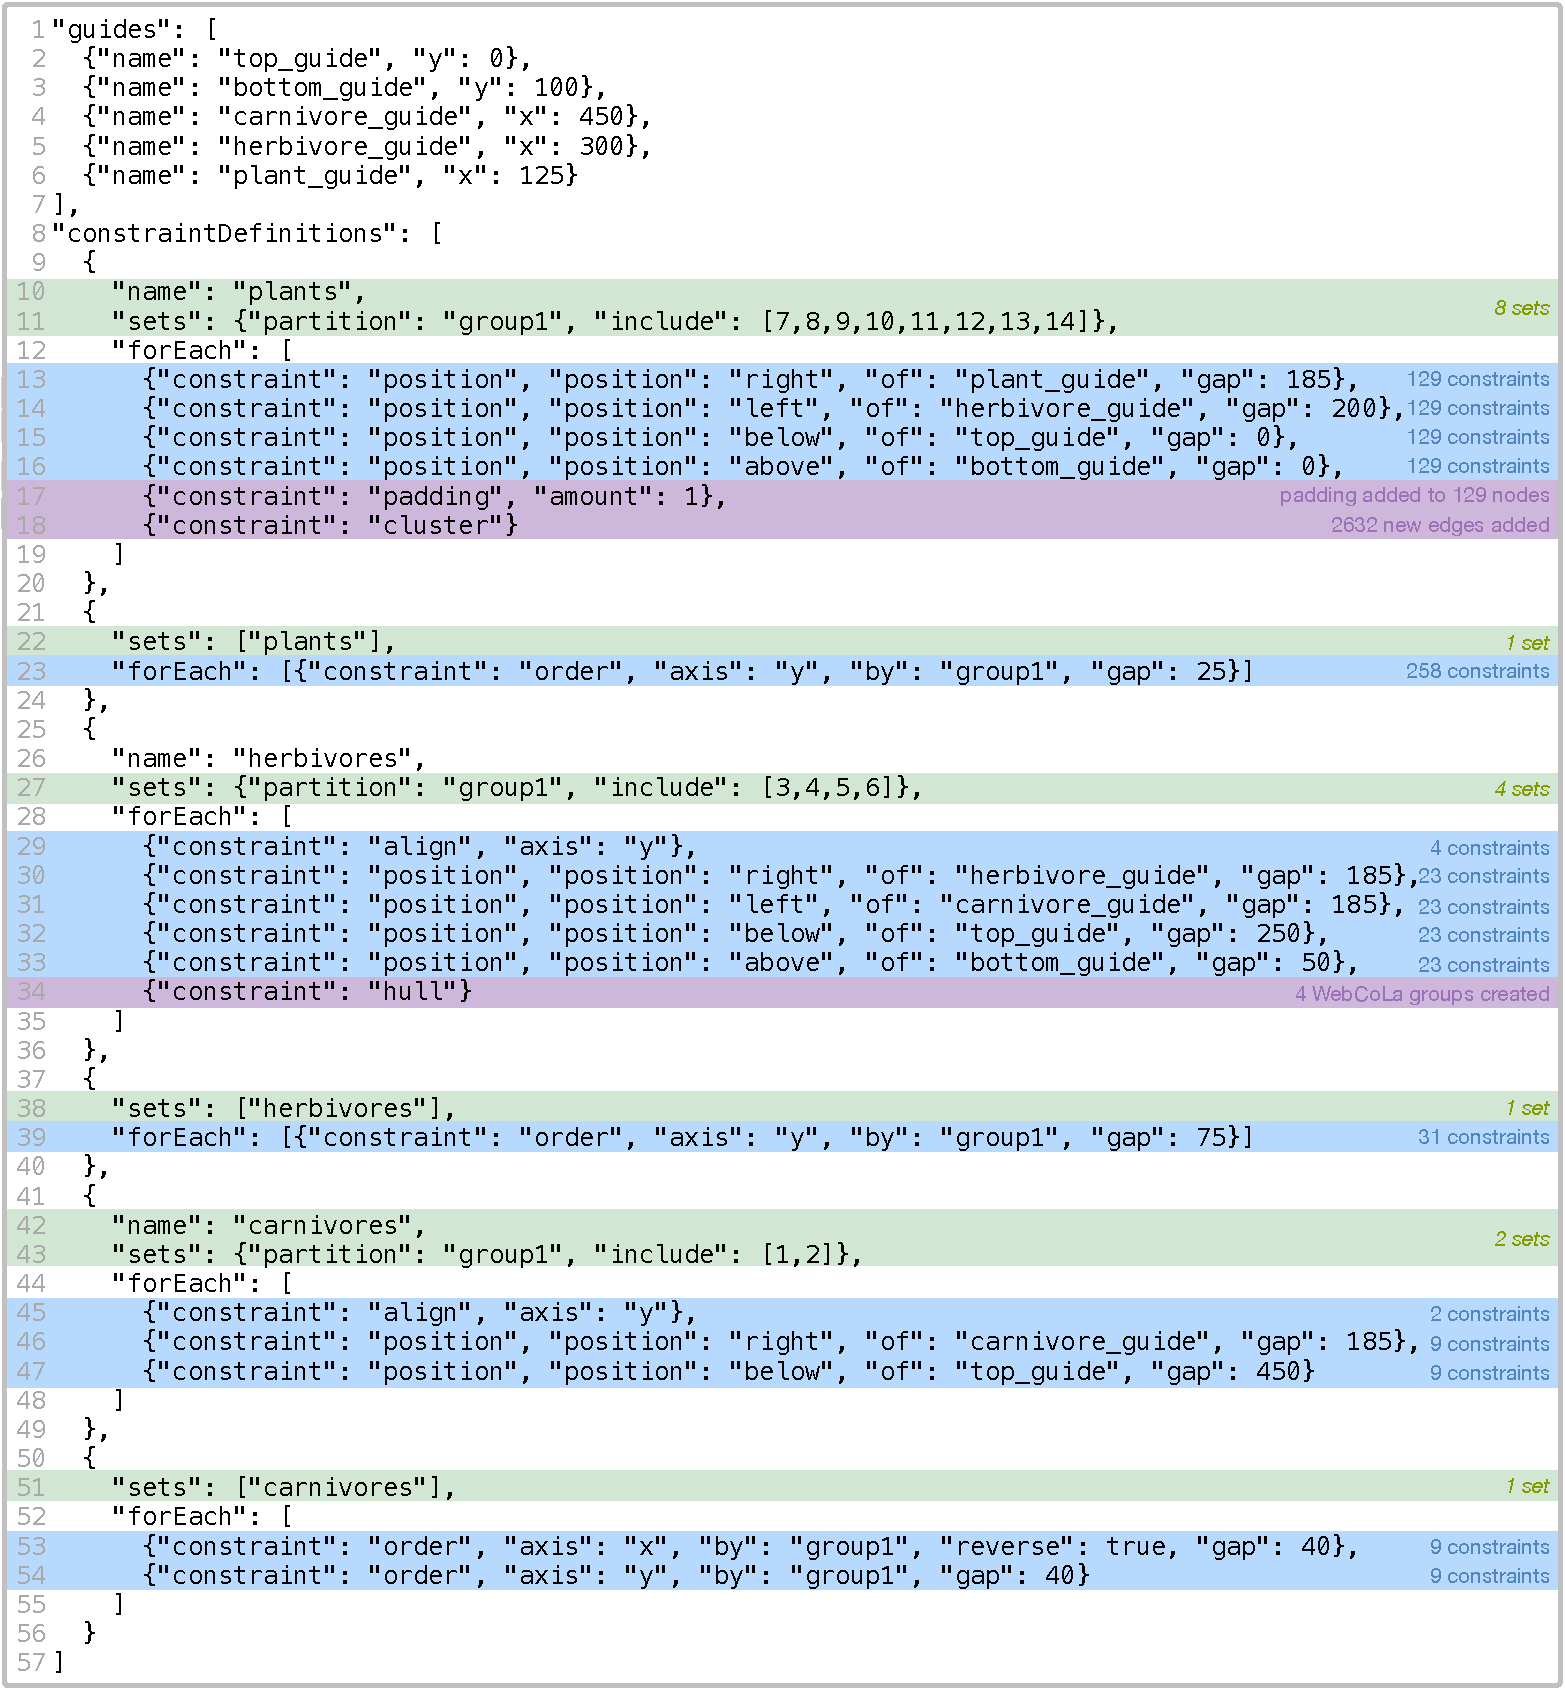
\includegraphics[width=\columnwidth]{figures/serengeti-spec.pdf}
    \vspace{-20px} {\caption{\label{fig:serengeti-spec} The
        \projectname~specification for the Serengeti food web shown in
        Figure~\ref{fig:serengeti-layout}. The code is annotated with the
        number of sets produced, the number of edges added, and the number
        of WebCoLa constraints generated for the final layout.}}
  \end{figure}
}

\newcommand{\syphilisLayout}{
  \begin{figure*}[t]
    \centering
    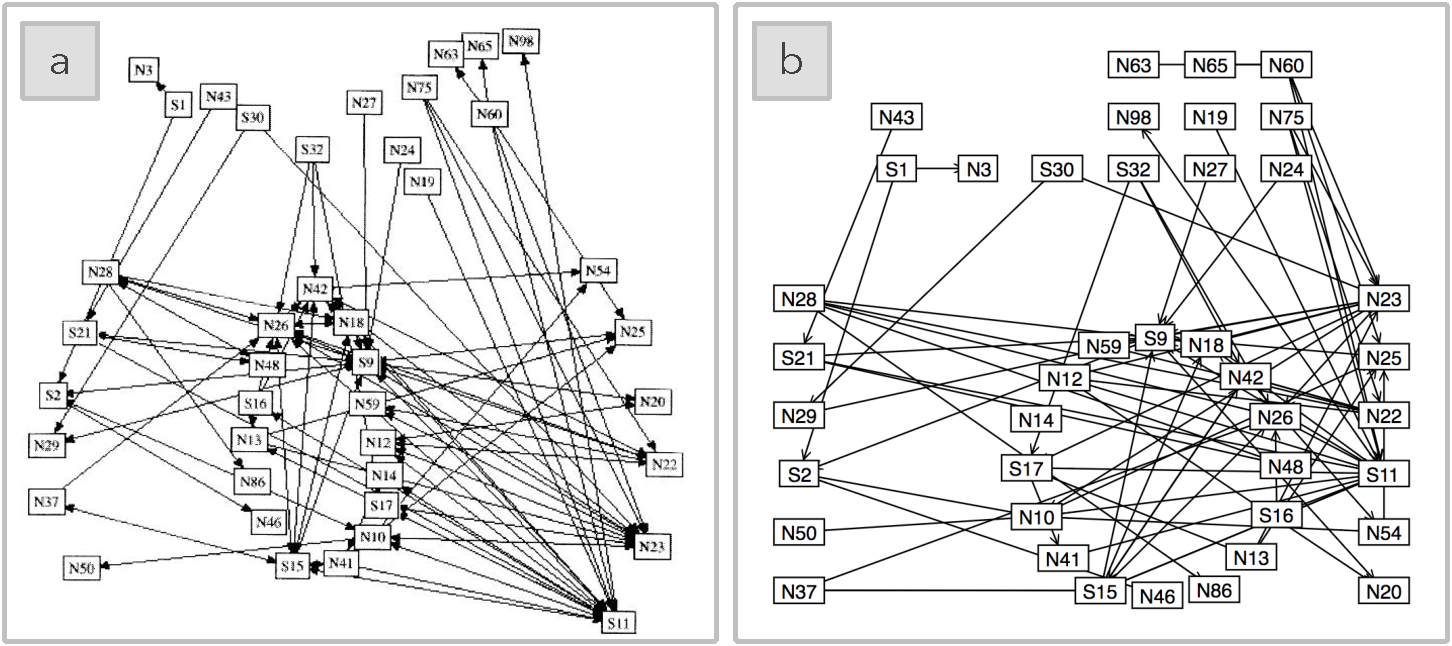
\includegraphics[width=\textwidth]{figures/syphilis-layout.pdf}
    \vspace{-20px} {\caption{\label{fig:syphilis-layout} The layout for the
        syphilis social network from (a) Rothenberg et
        al. \cite{rothenberg1998using} as compared to (b) the
        \projectname~layout. \todo{add some padding on the layout of the
          aligned men}}}
  \end{figure*}
}

\newcommand{\syphilisSpec}{
  \begin{figure}[t]
    \centering
    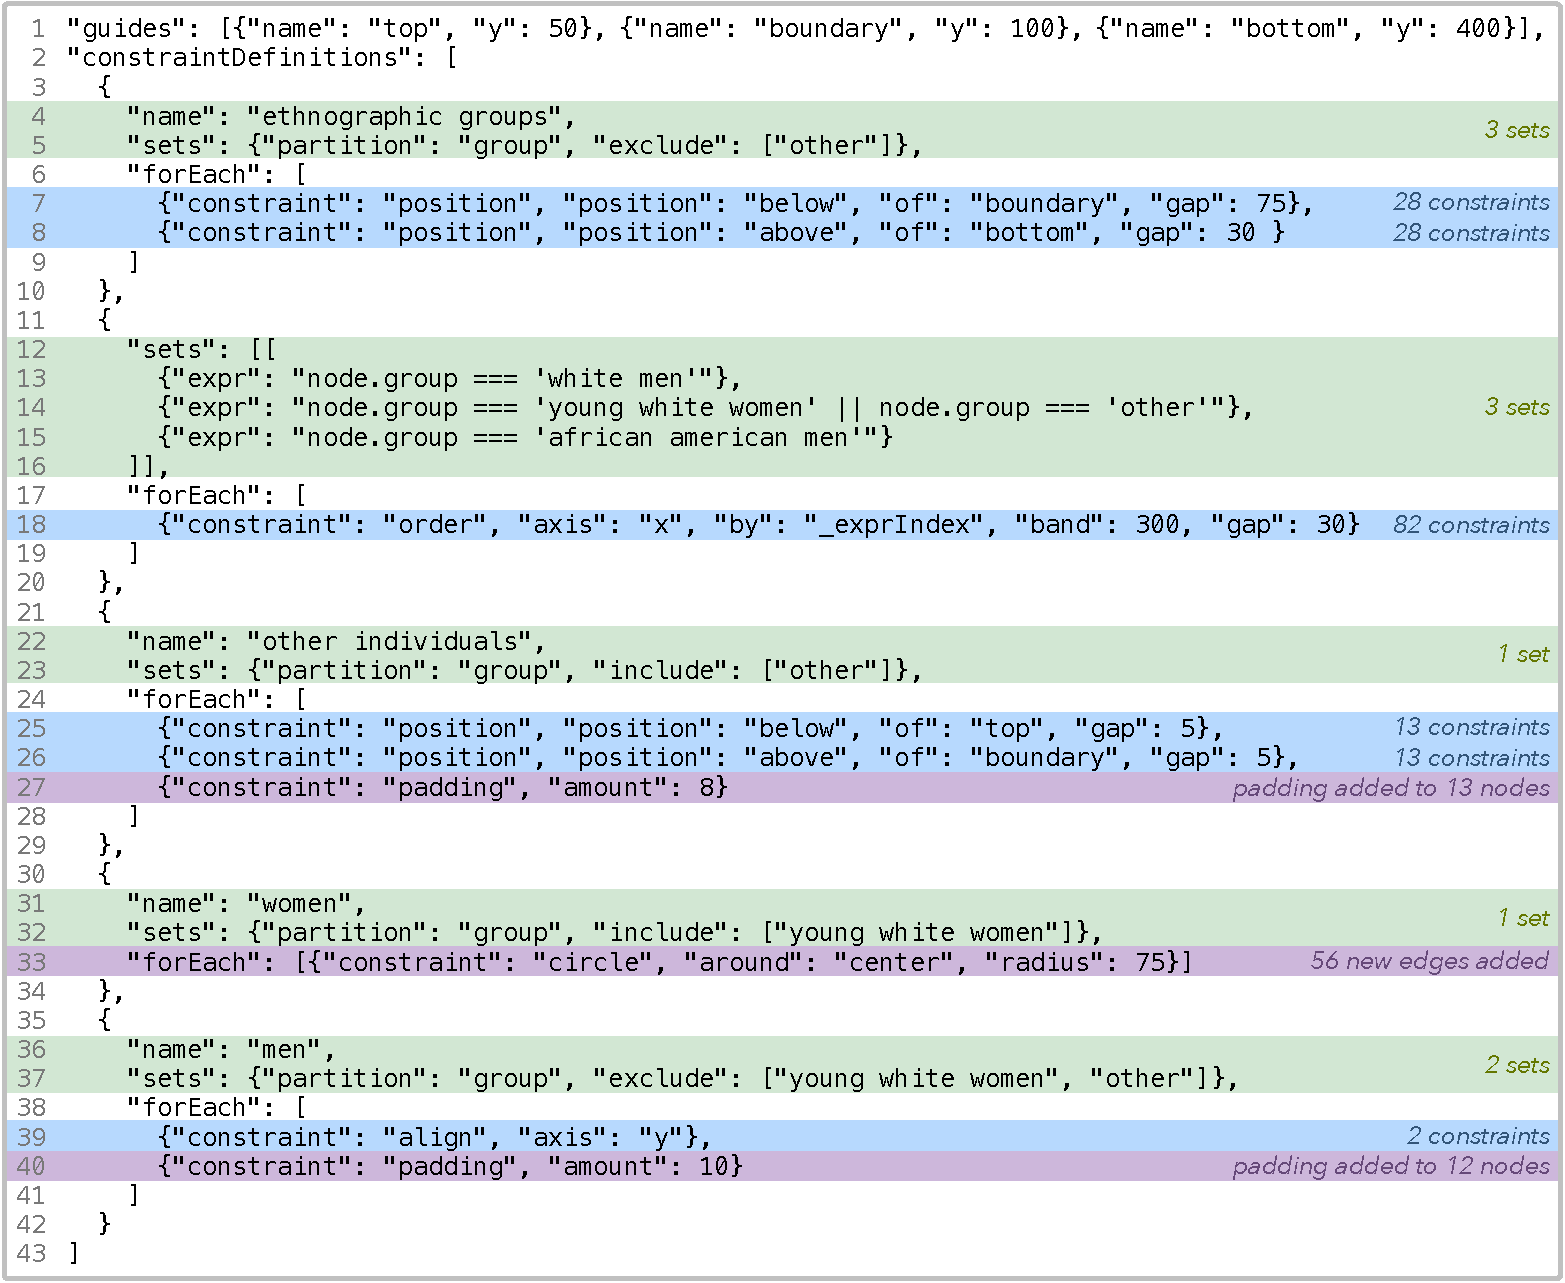
\includegraphics[width=\columnwidth]{figures/syphilis-spec.pdf}
    \vspace{-20px} {\caption{\label{fig:syphilis-spec} The
        \projectname~specification for the syphilis social network shown in
        Figure~\ref{fig:syphilis-layout}. The code is annotated with the
        number of sets produced, the number of edges added, and the number
        of WebCoLa constraints generated for the final layout.}}
  \end{figure}
}
